
%----------------------------------------------------------------
%----------------------------------------------------------------
\begin{frame}{Gas network model (recall)}   
\begin{figure}
    \begin{tikzpicture}
    \node[anchor=south west,inner sep=0] (X) at (-2, -3) 
    {\resizebox{0.95\textwidth}{!}{
    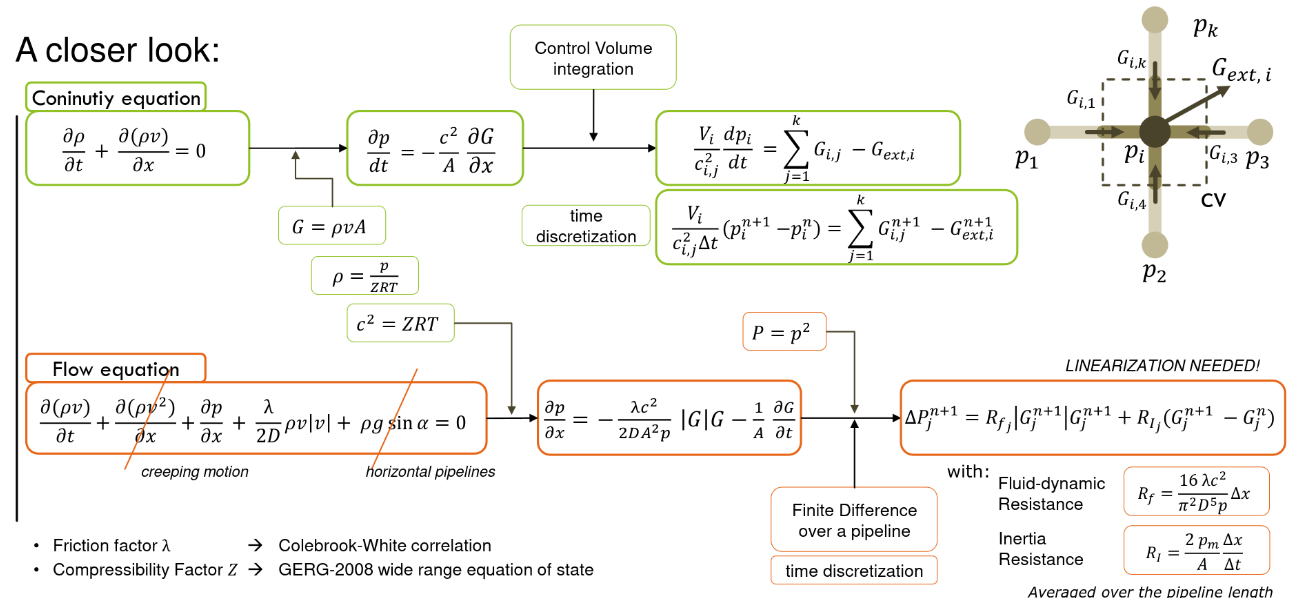
\includegraphics[scale = 1]{img_code/Marco_network_model.png}
    }};
    \node [blue, ultra thick] at ($(X.south west)!0.5!(X.north east)$) {};
    % Square for scale 0.4
    %\draw[red] (9.75,-3) -- (9.75,1.25) -- (4.0,1.25) -- (4.0,-3) -- cycle;
    % Square for scale 0.5
    \pgfsetfillcolor{lnode}
    \pgfsetfillopacity{0.5}
    \only<2->\fill(8.35,0.41) -- (8.35,1.15) -- (4.7,1.15) -- (4.7,0.41) -- cycle;
    \pgfsetfillcolor{lpipe}
    \pgfsetfillopacity{0.5}
    \only<3>\fill(7.2,-1.52) -- (7.2,-0.748) -- (11.1,-0.748) -- (11.1,-1.52) -- cycle;
    \end{tikzpicture}
    \caption{Taken from Marco's presentation.}
\end{figure}   
\end{frame}
%----------------------------------------------------------------
%----------------------------------------------------------------
\begin{frame}[fragile]{Linearized fluid-dynamic solver}

\begin{itemize}
    \item Code implementation mimics the system

\begin{minipage}{0.43\textwidth}
\begin{minted}[linenos=true,numbersep=1pt,frame=lines,framesep=2mm,fontsize=\notsotiny, escapeinside=||, bgcolor=background]{cpp}
void linearized_fluid_solver(){
 for(size_t iter=0;iter<=MAX_ITERS;iter++){    
    auto mass_system = |\cnodes{continuity}|( dt, ...);
    auto mom_system  = |\cpipes{momentum}|(dt, ...);
    auto bnd_system  = |\cbound{boundary}|(...);
        
    auto [LHS, rhs]= assemble(mass_system,
                               mom_system,
                       bnd_system, graph);

    solver.compute(LHS);
    vector_t sol = solver.solve(rhs);

    if(residual < tolerance)
       return;
 }}
\end{minted}
\end{minipage}%
\hfill
\begin{minipage}{0.45\textwidth}
    % Graphic for TeX using PGF
% Title: /home/karol/Documents/UNIVERSITA/POLITO/PRESENTATIONS/SHIMMER_2024_01/img_code/fluid_system.dia
% Creator: Dia v0.97.3
% CreationDate: Wed Jan 24 00:09:28 2024
% For: karol
% \usepackage{tikz}
% The following commands are not supported in PSTricks at present
% We define them conditionally, so when they are implemented,
% this pgf file will use them.
\ifx\du\undefined
  \newlength{\du}
\fi
\setlength{\du}{12\unitlength}
\begin{tikzpicture}[even odd rule]
\pgftransformxscale{1.000000}
\pgftransformyscale{-1.000000}
\definecolor{dialinecolor}{rgb}{0.000000, 0.000000, 0.000000}
\pgfsetstrokecolor{dialinecolor}
\pgfsetstrokeopacity{1.000000}
\definecolor{diafillcolor}{rgb}{1.000000, 1.000000, 1.000000}
\pgfsetfillcolor{diafillcolor}
\pgfsetfillopacity{1.000000}
\pgfsetlinewidth{0.050000\du}
\pgfsetdash{}{0pt}
\pgfsetmiterjoin
\pgfsetbuttcap
{\pgfsetcornersarced{\pgfpoint{0.000000\du}{0.000000\du}}\definecolor{dialinecolor}{rgb}{0.749020, 0.749020, 0.749020}
\pgfsetstrokecolor{dialinecolor}
\pgfsetstrokeopacity{1.000000}
\draw (25.200000\du,6.600000\du)--(25.200000\du,16.600000\du)--(27.500000\du,16.600000\du)--(27.500000\du,6.600000\du)--cycle;
}\pgfsetlinewidth{0.050000\du}
\pgfsetdash{}{0pt}
\pgfsetmiterjoin
\pgfsetbuttcap
{\pgfsetcornersarced{\pgfpoint{0.000000\du}{0.000000\du}}\definecolor{dialinecolor}{rgb}{0.749020, 0.749020, 0.749020}
\pgfsetstrokecolor{dialinecolor}
\pgfsetstrokeopacity{1.000000}
\draw (21.800000\du,6.600000\du)--(21.800000\du,16.600000\du)--(24.100000\du,16.600000\du)--(24.100000\du,6.600000\du)--cycle;
}\pgfsetlinewidth{0.050000\du}
\pgfsetdash{}{0pt}
\pgfsetmiterjoin
\pgfsetbuttcap
{\pgfsetcornersarced{\pgfpoint{0.000000\du}{0.000000\du}}\definecolor{dialinecolor}{rgb}{0.749020, 0.749020, 0.749020}
\pgfsetstrokecolor{dialinecolor}
\pgfsetstrokeopacity{1.000000}
\draw (11.500000\du,6.600000\du)--(11.500000\du,16.600000\du)--(21.400000\du,16.600000\du)--(21.400000\du,6.600000\du)--cycle;
}\pgfsetlinewidth{0.050000\du}
\pgfsetdash{}{0pt}
\pgfsetmiterjoin
{\pgfsetcornersarced{\pgfpoint{0.000000\du}{0.000000\du}}\definecolor{diafillcolor}{rgb}{0.882353, 0.803922, 0.882353}
\pgfsetfillcolor{lnode}
\pgfsetfillopacity{1.000000}
\fill (11.900000\du,7.000000\du)--(11.900000\du,10.000000\du)--(14.900000\du,10.000000\du)--(14.900000\du,7.000000\du)--cycle;
}{\pgfsetcornersarced{\pgfpoint{0.000000\du}{0.000000\du}}\definecolor{dialinecolor}{rgb}{0.749020, 0.749020, 0.749020}
\pgfsetstrokecolor{dialinecolor}
\pgfsetstrokeopacity{1.000000}
\draw (11.900000\du,7.000000\du)--(11.900000\du,10.000000\du)--(14.900000\du,10.000000\du)--(14.900000\du,7.000000\du)--cycle;
}% setfont left to latex
% setfont left to latex
\definecolor{dialinecolor}{rgb}{0.000000, 0.000000, 0.000000}
\pgfsetstrokecolor{dialinecolor}
\pgfsetstrokeopacity{1.000000}
\definecolor{diafillcolor}{rgb}{0.000000, 0.000000, 0.000000}
\pgfsetfillcolor{diafillcolor}
\pgfsetfillopacity{1.000000}
\node[anchor=base,inner sep=0pt, outer sep=0pt,color=dialinecolor] at (13.400000\du,8.785000\du){$\Phi$};
\pgfsetlinewidth{0.050000\du}
\pgfsetdash{}{0pt}
\pgfsetbuttcap
{
\definecolor{diafillcolor}{rgb}{0.666667, 0.670588, 0.670588}
\pgfsetfillcolor{diafillcolor}
\pgfsetfillopacity{1.000000}
% was here!!!
\definecolor{dialinecolor}{rgb}{0.666667, 0.670588, 0.670588}
\pgfsetstrokecolor{dialinecolor}
\pgfsetstrokeopacity{1.000000}
\draw (11.900000\du,7.000000\du)--(14.900000\du,10.000000\du);
}
\pgfsetlinewidth{0.050000\du}
\pgfsetdash{}{0pt}
\pgfsetmiterjoin
{\pgfsetcornersarced{\pgfpoint{0.000000\du}{0.000000\du}}\definecolor{diafillcolor}{rgb}{0.882353, 0.803922, 0.882353}
\pgfsetfillcolor{lnode}
\pgfsetfillopacity{1.000000}
\fill (15.300000\du,7.000000\du)--(15.300000\du,10.000000\du)--(17.600000\du,10.000000\du)--(17.600000\du,7.000000\du)--cycle;
}{\pgfsetcornersarced{\pgfpoint{0.000000\du}{0.000000\du}}\definecolor{dialinecolor}{rgb}{0.749020, 0.749020, 0.749020}
\pgfsetstrokecolor{dialinecolor}
\pgfsetstrokeopacity{1.000000}
\draw (15.300000\du,7.000000\du)--(15.300000\du,10.000000\du)--(17.600000\du,10.000000\du)--(17.600000\du,7.000000\du)--cycle;
}% setfont left to latex
% setfont left to latex
\definecolor{dialinecolor}{rgb}{0.000000, 0.000000, 0.000000}
\pgfsetstrokecolor{dialinecolor}
\pgfsetstrokeopacity{1.000000}
\definecolor{diafillcolor}{rgb}{0.000000, 0.000000, 0.000000}
\pgfsetfillcolor{diafillcolor}
\pgfsetfillopacity{1.000000}
\node[anchor=base,inner sep=0pt, outer sep=0pt,color=dialinecolor] at (16.450000\du,8.785000\du){$\mathbf{A}$};
\pgfsetlinewidth{0.050000\du}
\pgfsetdash{}{0pt}
\pgfsetmiterjoin
{\pgfsetcornersarced{\pgfpoint{0.000000\du}{0.000000\du}}\definecolor{diafillcolor}{rgb}{0.882353, 0.803922, 0.882353}
\pgfsetfillcolor{lnode}
\pgfsetfillopacity{1.000000}
\fill (18.000000\du,7.000000\du)--(18.000000\du,10.000000\du)--(21.000000\du,10.000000\du)--(21.000000\du,7.000000\du)--cycle;
}{\pgfsetcornersarced{\pgfpoint{0.000000\du}{0.000000\du}}\definecolor{dialinecolor}{rgb}{0.749020, 0.749020, 0.749020}
\pgfsetstrokecolor{dialinecolor}
\pgfsetstrokeopacity{1.000000}
\draw (18.000000\du,7.000000\du)--(18.000000\du,10.000000\du)--(21.000000\du,10.000000\du)--(21.000000\du,7.000000\du)--cycle;
}% setfont left to latex
% setfont left to latex
\definecolor{dialinecolor}{rgb}{0.000000, 0.000000, 0.000000}
\pgfsetstrokecolor{dialinecolor}
\pgfsetstrokeopacity{1.000000}
\definecolor{diafillcolor}{rgb}{0.000000, 0.000000, 0.000000}
\pgfsetfillcolor{diafillcolor}
\pgfsetfillopacity{1.000000}
\node[anchor=base,inner sep=0pt, outer sep=0pt,color=dialinecolor] at (19.500000\du,8.785000\du){{$\mathbf{I}$}};
\pgfsetlinewidth{0.050000\du}
\pgfsetdash{}{0pt}
\pgfsetbuttcap
{
\definecolor{diafillcolor}{rgb}{0.666667, 0.670588, 0.670588}
\pgfsetfillcolor{diafillcolor}
\pgfsetfillopacity{1.000000}
% was here!!!
\definecolor{dialinecolor}{rgb}{0.666667, 0.670588, 0.670588}
\pgfsetstrokecolor{dialinecolor}
\pgfsetstrokeopacity{1.000000}
\draw (18.000000\du,7.000000\du)--(21.000000\du,10.000000\du);
}
\pgfsetlinewidth{0.050000\du}
\pgfsetdash{}{0pt}
\pgfsetmiterjoin
{\pgfsetcornersarced{\pgfpoint{0.000000\du}{0.000000\du}}\definecolor{diafillcolor}{rgb}{0.882353, 0.803922, 0.882353}
\pgfsetfillcolor{lnode}
\pgfsetfillopacity{1.000000}
\fill (22.222183\du,7.000000\du)--(22.222183\du,10.000000\du)--(23.700000\du,10.000000\du)--(23.700000\du,7.000000\du)--cycle;
}{\pgfsetcornersarced{\pgfpoint{0.000000\du}{0.000000\du}}\definecolor{dialinecolor}{rgb}{0.749020, 0.749020, 0.749020}
\pgfsetstrokecolor{dialinecolor}
\pgfsetstrokeopacity{1.000000}
\draw (22.222183\du,7.000000\du)--(22.222183\du,10.000000\du)--(23.700000\du,10.000000\du)--(23.700000\du,7.000000\du)--cycle;
}% setfont left to latex
% setfont left to latex
\definecolor{dialinecolor}{rgb}{0.000000, 0.000000, 0.000000}
\pgfsetstrokecolor{dialinecolor}
\pgfsetstrokeopacity{1.000000}
\definecolor{diafillcolor}{rgb}{0.000000, 0.000000, 0.000000}
\pgfsetfillcolor{diafillcolor}
\pgfsetfillopacity{1.000000}
\node[anchor=base,inner sep=0pt, outer sep=0pt,color=dialinecolor] at (22.961092\du,8.785000\du){$\mathbf{p}$};
\pgfsetlinewidth{0.050000\du}
\pgfsetdash{}{0pt}
\pgfsetmiterjoin
{\pgfsetcornersarced{\pgfpoint{0.000000\du}{0.000000\du}}\definecolor{diafillcolor}{rgb}{0.882353, 0.803922, 0.882353}
\pgfsetfillcolor{lnode}
\pgfsetfillopacity{1.000000}
\fill (25.600000\du,7.000000\du)--(25.600000\du,10.000000\du)--(27.100000\du,10.000000\du)--(27.100000\du,7.000000\du)--cycle;
}{\pgfsetcornersarced{\pgfpoint{0.000000\du}{0.000000\du}}\definecolor{dialinecolor}{rgb}{0.749020, 0.749020, 0.749020}
\pgfsetstrokecolor{dialinecolor}
\pgfsetstrokeopacity{1.000000}
\draw (25.600000\du,7.000000\du)--(25.600000\du,10.000000\du)--(27.100000\du,10.000000\du)--(27.100000\du,7.000000\du)--cycle;
}% setfont left to latex
% setfont left to latex
\definecolor{dialinecolor}{rgb}{0.000000, 0.000000, 0.000000}
\pgfsetstrokecolor{dialinecolor}
\pgfsetstrokeopacity{1.000000}
\definecolor{diafillcolor}{rgb}{0.000000, 0.000000, 0.000000}
\pgfsetfillcolor{diafillcolor}
\pgfsetfillopacity{1.000000}
\node[anchor=base,inner sep=0pt, outer sep=0pt,color=dialinecolor] at (26.350000\du,8.785000\du){$\mathbf{F}_p$};
\pgfsetlinewidth{0.050000\du}
\pgfsetdash{}{0pt}
\pgfsetmiterjoin
{\pgfsetcornersarced{\pgfpoint{0.000000\du}{0.000000\du}}\definecolor{diafillcolor}{rgb}{0.847059, 0.898039, 0.898039}
\pgfsetfillcolor{lpipe}
\pgfsetfillopacity{1.000000}
\fill (11.900000\du,10.400000\du)--(11.900000\du,12.700000\du)--(14.900000\du,12.700000\du)--(14.900000\du,10.400000\du)--cycle;
}{\pgfsetcornersarced{\pgfpoint{0.000000\du}{0.000000\du}}\definecolor{dialinecolor}{rgb}{0.749020, 0.749020, 0.749020}
\pgfsetstrokecolor{dialinecolor}
\pgfsetstrokeopacity{1.000000}
\draw (11.900000\du,10.400000\du)--(11.900000\du,12.700000\du)--(14.900000\du,12.700000\du)--(14.900000\du,10.400000\du)--cycle;
}% setfont left to latex
% setfont left to latex
\definecolor{dialinecolor}{rgb}{0.000000, 0.000000, 0.000000}
\pgfsetstrokecolor{dialinecolor}
\pgfsetstrokeopacity{1.000000}
\definecolor{diafillcolor}{rgb}{0.000000, 0.000000, 0.000000}
\pgfsetfillcolor{diafillcolor}
\pgfsetfillopacity{1.000000}
\node[anchor=base,inner sep=0pt, outer sep=0pt,color=dialinecolor] at (13.400000\du,11.835000\du){$\mathbf{A}_{DP}$};
\pgfsetlinewidth{0.050000\du}
\pgfsetdash{}{0pt}
\pgfsetmiterjoin
{\pgfsetcornersarced{\pgfpoint{0.000000\du}{0.000000\du}}\definecolor{diafillcolor}{rgb}{0.847059, 0.898039, 0.898039}
\pgfsetfillcolor{lpipe}
\pgfsetfillopacity{1.000000}
\fill (15.300000\du,10.400000\du)--(15.300000\du,12.700000\du)--(17.600000\du,12.700000\du)--(17.600000\du,10.400000\du)--cycle;
}{\pgfsetcornersarced{\pgfpoint{0.000000\du}{0.000000\du}}\definecolor{dialinecolor}{rgb}{0.749020, 0.749020, 0.749020}
\pgfsetstrokecolor{dialinecolor}
\pgfsetstrokeopacity{1.000000}
\draw (15.300000\du,10.400000\du)--(15.300000\du,12.700000\du)--(17.600000\du,12.700000\du)--(17.600000\du,10.400000\du)--cycle;
}% setfont left to latex
% setfont left to latex
\definecolor{dialinecolor}{rgb}{0.000000, 0.000000, 0.000000}
\pgfsetstrokecolor{dialinecolor}
\pgfsetstrokeopacity{1.000000}
\definecolor{diafillcolor}{rgb}{0.000000, 0.000000, 0.000000}
\pgfsetfillcolor{diafillcolor}
\pgfsetfillopacity{1.000000}
\node[anchor=base,inner sep=0pt, outer sep=0pt,color=dialinecolor] at (16.450000\du,11.835000\du){{$-\mathbf{R}$}};
\pgfsetlinewidth{0.050000\du}
\pgfsetdash{}{0pt}
\pgfsetbuttcap
{
\definecolor{diafillcolor}{rgb}{0.666667, 0.670588, 0.670588}
\pgfsetfillcolor{diafillcolor}
\pgfsetfillopacity{1.000000}
% was here!!!
\definecolor{dialinecolor}{rgb}{0.666667, 0.670588, 0.670588}
\pgfsetstrokecolor{dialinecolor}
\pgfsetstrokeopacity{1.000000}
\draw (15.300000\du,10.400000\du)--(17.600000\du,12.700000\du);
}
\pgfsetlinewidth{0.050000\du}
\pgfsetdash{}{0pt}
\pgfsetmiterjoin
{\pgfsetcornersarced{\pgfpoint{0.000000\du}{0.000000\du}}\definecolor{diafillcolor}{rgb}{0.847059, 0.898039, 0.898039}
\pgfsetfillcolor{lpipe}
\pgfsetfillopacity{1.000000}
\fill (18.000000\du,10.400000\du)--(18.000000\du,12.700000\du)--(21.000000\du,12.700000\du)--(21.000000\du,10.400000\du)--cycle;
}{\pgfsetcornersarced{\pgfpoint{0.000000\du}{0.000000\du}}\definecolor{dialinecolor}{rgb}{0.749020, 0.749020, 0.749020}
\pgfsetstrokecolor{dialinecolor}
\pgfsetstrokeopacity{1.000000}
\draw (18.000000\du,10.400000\du)--(18.000000\du,12.700000\du)--(21.000000\du,12.700000\du)--(21.000000\du,10.400000\du)--cycle;
}% setfont left to latex
% setfont left to latex
\definecolor{dialinecolor}{rgb}{0.000000, 0.000000, 0.000000}
\pgfsetstrokecolor{dialinecolor}
\pgfsetstrokeopacity{1.000000}
\definecolor{diafillcolor}{rgb}{0.000000, 0.000000, 0.000000}
\pgfsetfillcolor{diafillcolor}
\pgfsetfillopacity{1.000000}
\node[anchor=base,inner sep=0pt, outer sep=0pt,color=dialinecolor] at (19.500000\du,11.835000\du){{$\mathbf{0}$}};
\pgfsetlinewidth{0.050000\du}
\pgfsetdash{}{0pt}
\pgfsetmiterjoin
{\pgfsetcornersarced{\pgfpoint{0.000000\du}{0.000000\du}}\definecolor{diafillcolor}{rgb}{0.847059, 0.898039, 0.898039}
\pgfsetfillcolor{lpipe}
\pgfsetfillopacity{1.000000}
\fill (22.222183\du,10.400000\du)--(22.222183\du,12.700000\du)--(23.700000\du,12.700000\du)--(23.700000\du,10.400000\du)--cycle;
}{\pgfsetcornersarced{\pgfpoint{0.000000\du}{0.000000\du}}\definecolor{dialinecolor}{rgb}{0.749020, 0.749020, 0.749020}
\pgfsetstrokecolor{dialinecolor}
\pgfsetstrokeopacity{1.000000}
\draw (22.222183\du,10.400000\du)--(22.222183\du,12.700000\du)--(23.700000\du,12.700000\du)--(23.700000\du,10.400000\du)--cycle;
}% setfont left to latex
% setfont left to latex
\definecolor{dialinecolor}{rgb}{0.000000, 0.000000, 0.000000}
\pgfsetstrokecolor{dialinecolor}
\pgfsetstrokeopacity{1.000000}
\definecolor{diafillcolor}{rgb}{0.000000, 0.000000, 0.000000}
\pgfsetfillcolor{diafillcolor}
\pgfsetfillopacity{1.000000}
\node[anchor=base,inner sep=0pt, outer sep=0pt,color=dialinecolor] at (22.961092\du,11.835000\du){$\mathbf{G}$};
\pgfsetlinewidth{0.050000\du}
\pgfsetdash{}{0pt}
\pgfsetmiterjoin
{\pgfsetcornersarced{\pgfpoint{0.000000\du}{0.000000\du}}\definecolor{diafillcolor}{rgb}{0.847059, 0.898039, 0.898039}
\pgfsetfillcolor{lpipe}
\pgfsetfillopacity{1.000000}
\fill (25.600000\du,10.400000\du)--(25.600000\du,12.700000\du)--(27.100000\du,12.700000\du)--(27.100000\du,10.400000\du)--cycle;
}{\pgfsetcornersarced{\pgfpoint{0.000000\du}{0.000000\du}}\definecolor{dialinecolor}{rgb}{0.749020, 0.749020, 0.749020}
\pgfsetstrokecolor{dialinecolor}
\pgfsetstrokeopacity{1.000000}
\draw (25.600000\du,10.400000\du)--(25.600000\du,12.700000\du)--(27.100000\du,12.700000\du)--(27.100000\du,10.400000\du)--cycle;
}% setfont left to latex
% setfont left to latex
\definecolor{dialinecolor}{rgb}{0.000000, 0.000000, 0.000000}
\pgfsetstrokecolor{dialinecolor}
\pgfsetstrokeopacity{1.000000}
\definecolor{diafillcolor}{rgb}{1.000000, 1.000000, 1.000000}
\pgfsetfillcolor{diafillcolor}
\pgfsetfillopacity{1.000000}
\node[anchor=base,inner sep=0pt, outer sep=0pt,color=dialinecolor] at (26.350000\du,11.835000\du){$\mathbf{F}_G$};
\pgfsetlinewidth{0.050000\du}
\pgfsetdash{}{0pt}
\pgfsetmiterjoin
{\pgfsetcornersarced{\pgfpoint{0.000000\du}{0.000000\du}}\definecolor{diafillcolor}{rgb}{0.882353, 0.825071, 0.686107}
\pgfsetfillcolor{lbound}
\pgfsetfillopacity{1.000000}
\fill (11.900000\du,13.200000\du)--(11.900000\du,16.200000\du)--(14.900000\du,16.200000\du)--(14.900000\du,13.200000\du)--cycle;
}{\pgfsetcornersarced{\pgfpoint{0.000000\du}{0.000000\du}}\definecolor{dialinecolor}{rgb}{0.749020, 0.749020, 0.749020}
\pgfsetstrokecolor{dialinecolor}
\pgfsetstrokeopacity{1.000000}
\draw (11.900000\du,13.200000\du)--(11.900000\du,16.200000\du)--(14.900000\du,16.200000\du)--(14.900000\du,13.200000\du)--cycle;
}% setfont left to latex
% setfont left to latex
\definecolor{dialinecolor}{rgb}{0.000000, 0.000000, 0.000000}
\pgfsetstrokecolor{dialinecolor}
\pgfsetstrokeopacity{1.000000}
\definecolor{diafillcolor}{rgb}{0.000000, 0.000000, 0.000000}
\pgfsetfillcolor{diafillcolor}
\pgfsetfillopacity{1.000000}
\node[anchor=base,inner sep=0pt, outer sep=0pt,color=dialinecolor] at (13.400000\du,14.985000\du){};
\pgfsetlinewidth{0.100000\du}
\pgfsetdash{{\pgflinewidth}{0.200000\du}}{0cm}
\pgfsetbuttcap
{
\definecolor{diafillcolor}{rgb}{0.666667, 0.670588, 0.670588}
\pgfsetfillcolor{diafillcolor}
\pgfsetfillopacity{1.000000}
% was here!!!
\definecolor{dialinecolor}{rgb}{0.666667, 0.670588, 0.670588}
\pgfsetstrokecolor{dialinecolor}
\pgfsetstrokeopacity{1.000000}
\draw (11.900000\du,13.200000\du)--(14.900000\du,16.200000\du);
}
\pgfsetlinewidth{0.050000\du}
\pgfsetdash{}{0pt}
\pgfsetmiterjoin
{\pgfsetcornersarced{\pgfpoint{0.000000\du}{0.000000\du}}\definecolor{diafillcolor}{rgb}{0.882353, 0.825071, 0.686107}
\pgfsetfillcolor{lbound}
\pgfsetfillopacity{1.000000}
\fill (15.300000\du,13.200000\du)--(15.300000\du,16.200000\du)--(17.600000\du,16.200000\du)--(17.600000\du,13.200000\du)--cycle;
}{\pgfsetcornersarced{\pgfpoint{0.000000\du}{0.000000\du}}\definecolor{dialinecolor}{rgb}{0.749020, 0.749020, 0.749020}
\pgfsetstrokecolor{dialinecolor}
\pgfsetstrokeopacity{1.000000}
\draw (15.300000\du,13.200000\du)--(15.300000\du,16.200000\du)--(17.600000\du,16.200000\du)--(17.600000\du,13.200000\du)--cycle;
}% setfont left to latex
% setfont left to latex
\definecolor{dialinecolor}{rgb}{0.000000, 0.000000, 0.000000}
\pgfsetstrokecolor{dialinecolor}
\pgfsetstrokeopacity{1.000000}
\definecolor{diafillcolor}{rgb}{0.000000, 0.000000, 0.000000}
\pgfsetfillcolor{diafillcolor}
\pgfsetfillopacity{1.000000}
\node[anchor=base,inner sep=0pt, outer sep=0pt,color=dialinecolor] at (16.450000\du,14.985000\du){$\mathbf{0}$};
\pgfsetlinewidth{0.050000\du}
\pgfsetdash{}{0pt}
\pgfsetmiterjoin
{\pgfsetcornersarced{\pgfpoint{0.000000\du}{0.000000\du}}\definecolor{diafillcolor}{rgb}{0.882353, 0.825071, 0.686107}
\pgfsetfillcolor{lbound}
\pgfsetfillopacity{1.000000}
\fill (18.000000\du,13.200000\du)--(18.000000\du,16.200000\du)--(21.000000\du,16.200000\du)--(21.000000\du,13.200000\du)--cycle;
}{\pgfsetcornersarced{\pgfpoint{0.000000\du}{0.000000\du}}\definecolor{dialinecolor}{rgb}{0.749020, 0.749020, 0.749020}
\pgfsetstrokecolor{dialinecolor}
\pgfsetstrokeopacity{1.000000}
\draw (18.000000\du,13.200000\du)--(18.000000\du,16.200000\du)--(21.000000\du,16.200000\du)--(21.000000\du,13.200000\du)--cycle;
}% setfont left to latex
% setfont left to latex
\definecolor{dialinecolor}{rgb}{0.000000, 0.000000, 0.000000}
\pgfsetstrokecolor{dialinecolor}
\pgfsetstrokeopacity{1.000000}
\definecolor{diafillcolor}{rgb}{0.000000, 0.000000, 0.000000}
\pgfsetfillcolor{diafillcolor}
\pgfsetfillopacity{1.000000}
\node[anchor=base,inner sep=0pt, outer sep=0pt,color=dialinecolor] at (19.500000\du,14.985000\du){};
\pgfsetlinewidth{0.100000\du}
\pgfsetdash{{\pgflinewidth}{0.200000\du}}{0cm}
\pgfsetbuttcap
{
\definecolor{diafillcolor}{rgb}{0.666667, 0.670588, 0.670588}
\pgfsetfillcolor{diafillcolor}
\pgfsetfillopacity{1.000000}
% was here!!!
\definecolor{dialinecolor}{rgb}{0.666667, 0.670588, 0.670588}
\pgfsetstrokecolor{dialinecolor}
\pgfsetstrokeopacity{1.000000}
\draw (18.000000\du,13.200000\du)--(21.000000\du,16.200000\du);
}
\pgfsetlinewidth{0.050000\du}
\pgfsetdash{}{0pt}
\pgfsetmiterjoin
{\pgfsetcornersarced{\pgfpoint{0.000000\du}{0.000000\du}}\definecolor{diafillcolor}{rgb}{0.882353, 0.825071, 0.686107}
\pgfsetfillcolor{lbound}
\pgfsetfillopacity{1.000000}
\fill (22.222183\du,13.200000\du)--(22.222183\du,16.200000\du)--(23.700000\du,16.200000\du)--(23.700000\du,13.200000\du)--cycle;
}{\pgfsetcornersarced{\pgfpoint{0.000000\du}{0.000000\du}}\definecolor{dialinecolor}{rgb}{0.749020, 0.749020, 0.749020}
\pgfsetstrokecolor{dialinecolor}
\pgfsetstrokeopacity{1.000000}
\draw (22.222183\du,13.200000\du)--(22.222183\du,16.200000\du)--(23.700000\du,16.200000\du)--(23.700000\du,13.200000\du)--cycle;
}% setfont left to latex
% setfont left to latex
\definecolor{dialinecolor}{rgb}{0.000000, 0.000000, 0.000000}
\pgfsetstrokecolor{dialinecolor}
\pgfsetstrokeopacity{1.000000}
\definecolor{diafillcolor}{rgb}{0.000000, 0.000000, 0.000000}
\pgfsetfillcolor{diafillcolor}
\pgfsetfillopacity{1.000000}
\node[anchor=base,inner sep=0pt, outer sep=0pt,color=dialinecolor] at (22.961092\du,14.985000\du){$\mathbf{L}$};
\pgfsetlinewidth{0.050000\du}
\pgfsetdash{}{0pt}
\pgfsetmiterjoin
{\pgfsetcornersarced{\pgfpoint{0.000000\du}{0.000000\du}}\definecolor{diafillcolor}{rgb}{0.882353, 0.825071, 0.686107}
\pgfsetfillcolor{lbound}
\pgfsetfillopacity{1.000000}
\fill (25.600000\du,13.200000\du)--(25.600000\du,16.200000\du)--(27.100000\du,16.200000\du)--(27.100000\du,13.200000\du)--cycle;
}{\pgfsetcornersarced{\pgfpoint{0.000000\du}{0.000000\du}}\definecolor{dialinecolor}{rgb}{0.749020, 0.749020, 0.749020}
\pgfsetstrokecolor{dialinecolor}
\pgfsetstrokeopacity{1.000000}
\draw (25.600000\du,13.200000\du)--(25.600000\du,16.200000\du)--(27.100000\du,16.200000\du)--(27.100000\du,13.200000\du)--cycle;
}% setfont left to latex
% setfont left to latex
\definecolor{dialinecolor}{rgb}{0.000000, 0.000000, 0.000000}
\pgfsetstrokecolor{dialinecolor}
\pgfsetstrokeopacity{1.000000}
\definecolor{diafillcolor}{rgb}{0.000000, 0.000000, 0.000000}
\pgfsetfillcolor{diafillcolor}
\pgfsetfillopacity{1.000000}
\node[anchor=base,inner sep=0pt, outer sep=0pt,color=dialinecolor] at (26.350000\du,14.985000\du){$\mathbf{F}_b$};
% setfont left to latex
% setfont left to latex
\definecolor{dialinecolor}{rgb}{0.000000, 0.000000, 0.000000}
\pgfsetstrokecolor{dialinecolor}
\pgfsetstrokeopacity{1.000000}
\definecolor{diafillcolor}{rgb}{0.000000, 0.000000, 0.000000}
\pgfsetfillcolor{diafillcolor}
\pgfsetfillopacity{1.000000}
\node[anchor=base west,inner sep=0pt,outer sep=0pt,color=dialinecolor] at (24.400000\du,11.900000\du){=};
\pgfsetlinewidth{0.050000\du}
\pgfsetdash{}{0pt}
\pgfsetmiterjoin
{\pgfsetcornersarced{\pgfpoint{0.000000\du}{0.000000\du}}\definecolor{diafillcolor}{rgb}{0.898039, 0.898039, 0.898039}
\pgfsetfillcolor{diafillcolor}
\pgfsetfillopacity{1.000000}
\fill (28.054032\du,17.267559\du)--(28.054032\du,18.267559\du)--(29.054032\du,18.267559\du)--(29.054032\du,17.267559\du)--cycle;
}{\pgfsetcornersarced{\pgfpoint{0.000000\du}{0.000000\du}}\definecolor{dialinecolor}{rgb}{0.749020, 0.749020, 0.749020}
\pgfsetstrokecolor{dialinecolor}
\pgfsetstrokeopacity{1.000000}
\draw (28.054032\du,17.267559\du)--(28.054032\du,18.267559\du)--(29.054032\du,18.267559\du)--(29.054032\du,17.267559\du)--cycle;
}% setfont left to latex
% setfont left to latex
\definecolor{dialinecolor}{rgb}{0.000000, 0.000000, 0.000000}
\pgfsetstrokecolor{dialinecolor}
\pgfsetstrokeopacity{1.000000}
\definecolor{diafillcolor}{rgb}{0.000000, 0.000000, 0.000000}
\pgfsetfillcolor{diafillcolor}
\pgfsetfillopacity{1.000000}
\node[anchor=base,inner sep=0pt, outer sep=0pt,color=dialinecolor] at (22.554032\du,18.052559\du){};
\pgfsetlinewidth{0.050000\du}
\pgfsetdash{}{0pt}
\pgfsetbuttcap
{
\definecolor{diafillcolor}{rgb}{0.666667, 0.670588, 0.670588}
\pgfsetfillcolor{diafillcolor}
\pgfsetfillopacity{1.000000}
% was here!!!
\definecolor{dialinecolor}{rgb}{0.666667, 0.670588, 0.670588}
\pgfsetstrokecolor{dialinecolor}
\pgfsetstrokeopacity{1.000000}
\draw (28.054032\du,17.267559\du)--(29.054032\du,18.267559\du);
}
% setfont left to latex
% setfont left to latex
\definecolor{dialinecolor}{rgb}{0.000000, 0.000000, 0.000000}
\pgfsetstrokecolor{dialinecolor}
\pgfsetstrokeopacity{1.000000}
\definecolor{diafillcolor}{rgb}{0.000000, 0.000000, 0.000000}
\pgfsetfillcolor{diafillcolor}
\pgfsetfillopacity{1.000000}
\node[anchor=base west,inner sep=0pt,outer sep=0pt,color=dialinecolor] at (21.00000\du,18.000000\du){Diagonal matrix};
\end{tikzpicture}

\end{minipage}

\item Functions parameters:
\begin{minted}[linenos=true,numbersep=1pt,frame=lines,framesep=2mm,fontsize=\notsotiny,escapeinside=||, bgcolor=background]{cpp}
     |\cnodes{continuity}|( dt, Tm, pressure, pressure_old, incidence, graph, x_nodes, glaw_nodes);
     |\cpipes{momentum}|( dt, Tm, flux, flux_old, pressure, incidence, graph, x_pipes, glaw_pipes);
     |\cbound{boundary}|(p_in, vel, flux_ext, incidence, graph, inlet_nodes);
\end{minted}
\end{itemize}
\end{frame}
%----------------------------------------------------------------
%----------------------------------------------------------------
\begin{frame}[fragile]{Modified incidence matrix $\mathbf{A}_{DP}$}
\noindent
\begin{itemize}
    \setlength{\itemindent}{-2.em}
    \item Linearized momentum equation
    \begin{equation*}
        \fbox{$P_{j,in}^{k+1} - e^sP_{j,out}^{n+1}$} - (2R^k_{F,j}|G_j^{k}| + R_{I,j}) G_j^{k+1} = F_G(R_{I},R^k_F,G_j^{k})
    \end{equation*}
\end{itemize}

\begin{minipage}{0.465\textwidth}
with matrix form
\begin{center}
% Graphic for TeX using PGF
% Title: /home/karol/Documents/UNIVERSITA/POLITO/PRESENTATIONS/SHIMMER_2024_01/img_code/fluid_system_momentum_adp.dia
% Creator: Dia v0.97.3
% CreationDate: Wed Jan 24 15:42:32 2024
% For: karol
% \usepackage{tikz}
% The following commands are not supported in PSTricks at present
% We define them conditionally, so when they are implemented,
% this pgf file will use them.
\ifx\du\undefined
  \newlength{\du}
\fi
\setlength{\du}{10\unitlength}
\begin{tikzpicture}[even odd rule]
\pgftransformxscale{1.000000}
\pgftransformyscale{-1.000000}
\definecolor{dialinecolor}{rgb}{0.000000, 0.000000, 0.000000}
\pgfsetstrokecolor{dialinecolor}
\pgfsetstrokeopacity{1.000000}
\definecolor{diafillcolor}{rgb}{1.000000, 1.000000, 1.000000}
\pgfsetfillcolor{diafillcolor}
\pgfsetfillopacity{1.000000}
\pgfsetlinewidth{0.050000\du}
\pgfsetdash{}{0pt}
\pgfsetmiterjoin
{\pgfsetcornersarced{\pgfpoint{0.000000\du}{0.000000\du}}\definecolor{diafillcolor}{rgb}{0.882353, 0.803922, 0.882353}
\pgfsetfillcolor{diafillcolor}
\pgfsetfillopacity{1.000000}
\fill (12.400000\du,5.000000\du)--(12.400000\du,8.000000\du)--(13.877817\du,8.000000\du)--(13.877817\du,5.000000\du)--cycle;
}{\pgfsetcornersarced{\pgfpoint{0.000000\du}{0.000000\du}}\definecolor{dialinecolor}{rgb}{0.749020, 0.749020, 0.749020}
\pgfsetstrokecolor{dialinecolor}
\pgfsetstrokeopacity{1.000000}
\draw (12.400000\du,5.000000\du)--(12.400000\du,8.000000\du)--(13.877817\du,8.000000\du)--(13.877817\du,5.000000\du)--cycle;
}% setfont left to latex
% setfont left to latex
\definecolor{dialinecolor}{rgb}{0.000000, 0.000000, 0.000000}
\pgfsetstrokecolor{dialinecolor}
\pgfsetstrokeopacity{1.000000}
\definecolor{diafillcolor}{rgb}{0.000000, 0.000000, 0.000000}
\pgfsetfillcolor{diafillcolor}
\pgfsetfillopacity{1.000000}
\node[anchor=base,inner sep=0pt, outer sep=0pt,color=dialinecolor] at (13.138908\du,6.785000\du){$\mathbf{p}$};
\pgfsetlinewidth{0.050000\du}
\pgfsetdash{}{0pt}
\pgfsetmiterjoin
{\pgfsetcornersarced{\pgfpoint{0.000000\du}{0.000000\du}}\definecolor{diafillcolor}{rgb}{0.847059, 0.898039, 0.898039}
\pgfsetfillcolor{diafillcolor}
\pgfsetfillopacity{1.000000}
\fill (9.000000\du,5.000000\du)--(9.000000\du,7.300000\du)--(12.000000\du,7.300000\du)--(12.000000\du,5.000000\du)--cycle;
}{\pgfsetcornersarced{\pgfpoint{0.000000\du}{0.000000\du}}\definecolor{dialinecolor}{rgb}{1.000000, 0.000000, 0.000000}
\pgfsetstrokecolor{dialinecolor}
\pgfsetstrokeopacity{1.000000}
\draw (9.000000\du,5.000000\du)--(9.000000\du,7.300000\du)--(12.000000\du,7.300000\du)--(12.000000\du,5.000000\du)--cycle;
}% setfont left to latex
% setfont left to latex
\definecolor{dialinecolor}{rgb}{0.000000, 0.000000, 0.000000}
\pgfsetstrokecolor{dialinecolor}
\pgfsetstrokeopacity{1.000000}
\definecolor{diafillcolor}{rgb}{0.000000, 0.000000, 0.000000}
\pgfsetfillcolor{diafillcolor}
\pgfsetfillopacity{1.000000}
\node[anchor=base,inner sep=0pt, outer sep=0pt,color=dialinecolor] at (10.500000\du,6.435000\du){$\mathbf{A}_{DP}$};
\pgfsetlinewidth{0.050000\du}
\pgfsetdash{}{0pt}
\pgfsetmiterjoin
{\pgfsetcornersarced{\pgfpoint{0.000000\du}{0.000000\du}}\definecolor{diafillcolor}{rgb}{0.847059, 0.898039, 0.898039}
\pgfsetfillcolor{diafillcolor}
\pgfsetfillopacity{1.000000}
\fill (14.600000\du,5.000000\du)--(14.600000\du,7.300000\du)--(16.900000\du,7.300000\du)--(16.900000\du,5.000000\du)--cycle;
}{\pgfsetcornersarced{\pgfpoint{0.000000\du}{0.000000\du}}\definecolor{dialinecolor}{rgb}{0.749020, 0.749020, 0.749020}
\pgfsetstrokecolor{dialinecolor}
\pgfsetstrokeopacity{1.000000}
\draw (14.600000\du,5.000000\du)--(14.600000\du,7.300000\du)--(16.900000\du,7.300000\du)--(16.900000\du,5.000000\du)--cycle;
}% setfont left to latex
% setfont left to latex
\definecolor{dialinecolor}{rgb}{0.000000, 0.000000, 0.000000}
\pgfsetstrokecolor{dialinecolor}
\pgfsetstrokeopacity{1.000000}
\definecolor{diafillcolor}{rgb}{0.000000, 0.000000, 0.000000}
\pgfsetfillcolor{diafillcolor}
\pgfsetfillopacity{1.000000}
\node[anchor=base,inner sep=0pt, outer sep=0pt,color=dialinecolor] at (15.750000\du,6.435000\du){$\mathbf{R}$};
\pgfsetlinewidth{0.050000\du}
\pgfsetdash{}{0pt}
\pgfsetbuttcap
{
\definecolor{diafillcolor}{rgb}{0.666667, 0.670588, 0.670588}
\pgfsetfillcolor{diafillcolor}
\pgfsetfillopacity{1.000000}
% was here!!!
\definecolor{dialinecolor}{rgb}{0.666667, 0.670588, 0.670588}
\pgfsetstrokecolor{dialinecolor}
\pgfsetstrokeopacity{1.000000}
\draw (14.600000\du,5.000000\du)--(16.900000\du,7.300000\du);
}
\pgfsetlinewidth{0.050000\du}
\pgfsetdash{}{0pt}
\pgfsetmiterjoin
{\pgfsetcornersarced{\pgfpoint{0.000000\du}{0.000000\du}}\definecolor{diafillcolor}{rgb}{0.847059, 0.898039, 0.898039}
\pgfsetfillcolor{diafillcolor}
\pgfsetfillopacity{1.000000}
\fill (17.300000\du,5.000000\du)--(17.300000\du,7.300000\du)--(18.777817\du,7.300000\du)--(18.777817\du,5.000000\du)--cycle;
}{\pgfsetcornersarced{\pgfpoint{0.000000\du}{0.000000\du}}\definecolor{dialinecolor}{rgb}{0.749020, 0.749020, 0.749020}
\pgfsetstrokecolor{dialinecolor}
\pgfsetstrokeopacity{1.000000}
\draw (17.300000\du,5.000000\du)--(17.300000\du,7.300000\du)--(18.777817\du,7.300000\du)--(18.777817\du,5.000000\du)--cycle;
}% setfont left to latex
% setfont left to latex
\definecolor{dialinecolor}{rgb}{0.000000, 0.000000, 0.000000}
\pgfsetstrokecolor{dialinecolor}
\pgfsetstrokeopacity{1.000000}
\definecolor{diafillcolor}{rgb}{0.000000, 0.000000, 0.000000}
\pgfsetfillcolor{diafillcolor}
\pgfsetfillopacity{1.000000}
\node[anchor=base,inner sep=0pt, outer sep=0pt,color=dialinecolor] at (18.038908\du,6.435000\du){$\mathbf{G}$};
\pgfsetlinewidth{0.050000\du}
\pgfsetdash{}{0pt}
\pgfsetmiterjoin
{\pgfsetcornersarced{\pgfpoint{0.000000\du}{0.000000\du}}\definecolor{diafillcolor}{rgb}{0.847059, 0.898039, 0.898039}
\pgfsetfillcolor{diafillcolor}
\pgfsetfillopacity{1.000000}
\fill (19.500000\du,5.000000\du)--(19.500000\du,7.300000\du)--(21.000000\du,7.300000\du)--(21.000000\du,5.000000\du)--cycle;
}{\pgfsetcornersarced{\pgfpoint{0.000000\du}{0.000000\du}}\definecolor{dialinecolor}{rgb}{0.749020, 0.749020, 0.749020}
\pgfsetstrokecolor{dialinecolor}
\pgfsetstrokeopacity{1.000000}
\draw (19.500000\du,5.000000\du)--(19.500000\du,7.300000\du)--(21.000000\du,7.300000\du)--(21.000000\du,5.000000\du)--cycle;
}% setfont left to latex
% setfont left to latex
\definecolor{dialinecolor}{rgb}{0.000000, 0.000000, 0.000000}
\pgfsetstrokecolor{dialinecolor}
\pgfsetstrokeopacity{1.000000}
\definecolor{diafillcolor}{rgb}{0.000000, 0.000000, 0.000000}
\pgfsetfillcolor{diafillcolor}
\pgfsetfillopacity{1.000000}
\node[anchor=base,inner sep=0pt, outer sep=0pt,color=dialinecolor] at (20.250000\du,6.435000\du){$\mathbf{F_G}$};
% setfont left to latex
% setfont left to latex
\definecolor{dialinecolor}{rgb}{0.000000, 0.000000, 0.000000}
\pgfsetstrokecolor{dialinecolor}
\pgfsetstrokeopacity{1.000000}
\definecolor{diafillcolor}{rgb}{0.000000, 0.000000, 0.000000}
\pgfsetfillcolor{diafillcolor}
\pgfsetfillopacity{1.000000}
\node[anchor=base west,inner sep=0pt,outer sep=0pt,color=dialinecolor] at (18.8000000\du,6.300000\du){=};
% setfont left to latex
% setfont left to latex
\definecolor{dialinecolor}{rgb}{0.000000, 0.000000, 0.000000}
\pgfsetstrokecolor{dialinecolor}
\pgfsetstrokeopacity{1.000000}
\definecolor{diafillcolor}{rgb}{0.000000, 0.000000, 0.000000}
\pgfsetfillcolor{diafillcolor}
\pgfsetfillopacity{1.000000}
\node[anchor=base west,inner sep=0pt,outer sep=0pt,color=dialinecolor] at (13.961341\du,6.306816\du){-};
\end{tikzpicture}
     
\end{center}
\vspace{-0.5cm}
\begin{minted}[linenos=true,numbersep=1pt,frame=lines,framesep=2mm,fontsize=\notsotiny, bgcolor=background]{cpp}
smatrix_t
adp_matrix( const vector_t& c2, const my_graph& g,
            const incidence& inc)
{ 
   vector_t  exp_s = compute_expS(c2, g);
   smatrix_t sE = diag_matrix(exp_s);  

   smatrix_t ADP(num_edges(g),num_vertices(g));
   ADPt = inc.matrix_in() - inc.matrix_out()*sE;
   return ADPt.transpose();
}    
\end{minted}    
\end{minipage}
\hfill
\begin{minipage}{0.47\textwidth}
    \begin{minted}[linenos=true,numbersep=1pt,frame=lines,framesep=2mm,fontsize=\notsotiny, bgcolor=background]{cpp}
vector_t
compute_expS(const vector_t& c2, const my_graph& g)
{   
    vector_t  exp_s (num_edges(g)); 

    size_t i = 0;
    auto r = edges(g);
    for(auto it=r.first; it!=r.second; it++,i++)
    {
        auto pipe = g[*it];   
        auto node_in  = g[source(*it, g)];
        auto node_out = g[target(*it, g)];
        auto s = node_out.height - node_in.height;
        exp_s(i) =  std::exp(s * gravity / c2(i)); 
    }

    return exp_s;       
}
    \end{minted}
\end{minipage}
 \begin{tikzpicture}[remember picture,overlay]
\only<2>\draw[red] (-13.7,-1.56) -- (-13.7,-1.32) -- (-7.5,-1.32) -- (-7.5,-1.56) -- cycle;
 \end{tikzpicture}
\end{frame}
%----------------------------------------------------------------
%----------------------------------------------------------------

\begin{frame}[fragile]{Resistance matrix}
\noindent
%\hspace{-0.5cm}
\begin{minipage}{0.45\textwidth}
\begin{itemize}
    \setlength{\itemindent}{-2.em}
    \item Linearized momentum equation
\end{itemize}
    \noindent \hspace{-0.5cm}
    \[\small
        P_{j,in}^{k+1} - e^sP_{j,out}^{n+1} -\fbox{$(2R^k_{F,j}|G_j^{k}| + R_{I,j})$} G_j^{k+1} = F_G
    \]
    with matrix form 
    \begin{center}
    % Graphic for TeX using PGF
% Title: /home/karol/Documents/UNIVERSITA/POLITO/PRESENTATIONS/SHIMMER_2024_01/img_code/fluid_system_momentum_adp.dia
% Creator: Dia v0.97.3
% CreationDate: Thu Jan 25 10:36:14 2024
% For: karol
% \usepackage{tikz}
% The following commands are not supported in PSTricks at present
% We define them conditionally, so when they are implemented,
% this pgf file will use them.
\ifx\du\undefined
  \newlength{\du}
\fi
\setlength{\du}{10\unitlength}
\begin{tikzpicture}[even odd rule]
\pgftransformxscale{1.000000}
\pgftransformyscale{-1.000000}
\definecolor{dialinecolor}{rgb}{0.000000, 0.000000, 0.000000}
\pgfsetstrokecolor{dialinecolor}
\pgfsetstrokeopacity{1.000000}
\definecolor{diafillcolor}{rgb}{1.000000, 1.000000, 1.000000}
\pgfsetfillcolor{diafillcolor}
\pgfsetfillopacity{1.000000}
\pgfsetlinewidth{0.050000\du}
\pgfsetdash{}{0pt}
\pgfsetmiterjoin
{\pgfsetcornersarced{\pgfpoint{0.000000\du}{0.000000\du}}\definecolor{diafillcolor}{rgb}{0.882353, 0.803922, 0.882353}
\pgfsetfillcolor{diafillcolor}
\pgfsetfillopacity{1.000000}
\fill (12.400000\du,5.000000\du)--(12.400000\du,8.000000\du)--(13.877817\du,8.000000\du)--(13.877817\du,5.000000\du)--cycle;
}{\pgfsetcornersarced{\pgfpoint{0.000000\du}{0.000000\du}}\definecolor{dialinecolor}{rgb}{0.749020, 0.749020, 0.749020}
\pgfsetstrokecolor{dialinecolor}
\pgfsetstrokeopacity{1.000000}
\draw (12.400000\du,5.000000\du)--(12.400000\du,8.000000\du)--(13.877817\du,8.000000\du)--(13.877817\du,5.000000\du)--cycle;
}% setfont left to latex
% setfont left to latex
\definecolor{dialinecolor}{rgb}{0.000000, 0.000000, 0.000000}
\pgfsetstrokecolor{dialinecolor}
\pgfsetstrokeopacity{1.000000}
\definecolor{diafillcolor}{rgb}{0.000000, 0.000000, 0.000000}
\pgfsetfillcolor{diafillcolor}
\pgfsetfillopacity{1.000000}
\node[anchor=base,inner sep=0pt, outer sep=0pt,color=dialinecolor] at (13.138908\du,6.785000\du){$\mathbf{p}$};
\pgfsetlinewidth{0.050000\du}
\pgfsetdash{}{0pt}
\pgfsetmiterjoin
{\pgfsetcornersarced{\pgfpoint{0.000000\du}{0.000000\du}}\definecolor{diafillcolor}{rgb}{0.847059, 0.898039, 0.898039}
\pgfsetfillcolor{diafillcolor}
\pgfsetfillopacity{1.000000}
\fill (9.000000\du,5.000000\du)--(9.000000\du,7.300000\du)--(12.000000\du,7.300000\du)--(12.000000\du,5.000000\du)--cycle;
}{\pgfsetcornersarced{\pgfpoint{0.000000\du}{0.000000\du}}\definecolor{dialinecolor}{rgb}{0.666667, 0.670588, 0.670588}
\pgfsetstrokecolor{dialinecolor}
\pgfsetstrokeopacity{1.000000}
\draw (9.000000\du,5.000000\du)--(9.000000\du,7.300000\du)--(12.000000\du,7.300000\du)--(12.000000\du,5.000000\du)--cycle;
}% setfont left to latex
% setfont left to latex
\definecolor{dialinecolor}{rgb}{0.000000, 0.000000, 0.000000}
\pgfsetstrokecolor{dialinecolor}
\pgfsetstrokeopacity{1.000000}
\definecolor{diafillcolor}{rgb}{0.000000, 0.000000, 0.000000}
\pgfsetfillcolor{diafillcolor}
\pgfsetfillopacity{1.000000}
\node[anchor=base,inner sep=0pt, outer sep=0pt,color=dialinecolor] at (10.500000\du,6.435000\du){$\mathbf{A}_{DP}$};
\pgfsetlinewidth{0.050000\du}
\pgfsetdash{}{0pt}
\pgfsetmiterjoin
{\pgfsetcornersarced{\pgfpoint{0.000000\du}{0.000000\du}}\definecolor{diafillcolor}{rgb}{0.847059, 0.898039, 0.898039}
\pgfsetfillcolor{diafillcolor}
\pgfsetfillopacity{1.000000}
\fill (14.600000\du,5.000000\du)--(14.600000\du,7.300000\du)--(16.900000\du,7.300000\du)--(16.900000\du,5.000000\du)--cycle;
}{\pgfsetcornersarced{\pgfpoint{0.000000\du}{0.000000\du}}\definecolor{dialinecolor}{rgb}{1.000000, 0.000000, 0.000000}
\pgfsetstrokecolor{dialinecolor}
\pgfsetstrokeopacity{1.000000}
\draw (14.600000\du,5.000000\du)--(14.600000\du,7.300000\du)--(16.900000\du,7.300000\du)--(16.900000\du,5.000000\du)--cycle;
}% setfont left to latex
% setfont left to latex
\definecolor{dialinecolor}{rgb}{0.000000, 0.000000, 0.000000}
\pgfsetstrokecolor{dialinecolor}
\pgfsetstrokeopacity{1.000000}
\definecolor{diafillcolor}{rgb}{0.000000, 0.000000, 0.000000}
\pgfsetfillcolor{diafillcolor}
\pgfsetfillopacity{1.000000}
\node[anchor=base,inner sep=0pt, outer sep=0pt,color=dialinecolor] at (15.750000\du,6.435000\du){$\mathbf{R}$};
\pgfsetlinewidth{0.050000\du}
\pgfsetdash{}{0pt}
\pgfsetbuttcap
{
\definecolor{diafillcolor}{rgb}{0.666667, 0.670588, 0.670588}
\pgfsetfillcolor{diafillcolor}
\pgfsetfillopacity{1.000000}
% was here!!!
\definecolor{dialinecolor}{rgb}{0.666667, 0.670588, 0.670588}
\pgfsetstrokecolor{dialinecolor}
\pgfsetstrokeopacity{1.000000}
\draw (14.600000\du,5.000000\du)--(16.900000\du,7.300000\du);
}
\pgfsetlinewidth{0.050000\du}
\pgfsetdash{}{0pt}
\pgfsetmiterjoin
{\pgfsetcornersarced{\pgfpoint{0.000000\du}{0.000000\du}}\definecolor{diafillcolor}{rgb}{0.847059, 0.898039, 0.898039}
\pgfsetfillcolor{diafillcolor}
\pgfsetfillopacity{1.000000}
\fill (17.300000\du,5.000000\du)--(17.300000\du,7.300000\du)--(18.777817\du,7.300000\du)--(18.777817\du,5.000000\du)--cycle;
}{\pgfsetcornersarced{\pgfpoint{0.000000\du}{0.000000\du}}\definecolor{dialinecolor}{rgb}{0.749020, 0.749020, 0.749020}
\pgfsetstrokecolor{dialinecolor}
\pgfsetstrokeopacity{1.000000}
\draw (17.300000\du,5.000000\du)--(17.300000\du,7.300000\du)--(18.777817\du,7.300000\du)--(18.777817\du,5.000000\du)--cycle;
}% setfont left to latex
% setfont left to latex
\definecolor{dialinecolor}{rgb}{0.000000, 0.000000, 0.000000}
\pgfsetstrokecolor{dialinecolor}
\pgfsetstrokeopacity{1.000000}
\definecolor{diafillcolor}{rgb}{0.000000, 0.000000, 0.000000}
\pgfsetfillcolor{diafillcolor}
\pgfsetfillopacity{1.000000}
\node[anchor=base,inner sep=0pt, outer sep=0pt,color=dialinecolor] at (18.038908\du,6.435000\du){$\mathbf{G}$};
\pgfsetlinewidth{0.050000\du}
\pgfsetdash{}{0pt}
\pgfsetmiterjoin
{\pgfsetcornersarced{\pgfpoint{0.000000\du}{0.000000\du}}\definecolor{diafillcolor}{rgb}{0.847059, 0.898039, 0.898039}
\pgfsetfillcolor{diafillcolor}
\pgfsetfillopacity{1.000000}
\fill (19.500000\du,5.000000\du)--(19.500000\du,7.300000\du)--(21.000000\du,7.300000\du)--(21.000000\du,5.000000\du)--cycle;
}{\pgfsetcornersarced{\pgfpoint{0.000000\du}{0.000000\du}}\definecolor{dialinecolor}{rgb}{0.749020, 0.749020, 0.749020}
\pgfsetstrokecolor{dialinecolor}
\pgfsetstrokeopacity{1.000000}
\draw (19.500000\du,5.000000\du)--(19.500000\du,7.300000\du)--(21.000000\du,7.300000\du)--(21.000000\du,5.000000\du)--cycle;
}% setfont left to latex
% setfont left to latex
\definecolor{dialinecolor}{rgb}{0.000000, 0.000000, 0.000000}
\pgfsetstrokecolor{dialinecolor}
\pgfsetstrokeopacity{1.000000}
\definecolor{diafillcolor}{rgb}{0.000000, 0.000000, 0.000000}
\pgfsetfillcolor{diafillcolor}
\pgfsetfillopacity{1.000000}
\node[anchor=base,inner sep=0pt, outer sep=0pt,color=dialinecolor] at (20.250000\du,6.435000\du){$\mathbf{F_G}$};
% setfont left to latex
% setfont left to latex
\definecolor{dialinecolor}{rgb}{0.000000, 0.000000, 0.000000}
\pgfsetstrokecolor{dialinecolor}
\pgfsetstrokeopacity{1.000000}
\definecolor{diafillcolor}{rgb}{0.000000, 0.000000, 0.000000}
\pgfsetfillcolor{diafillcolor}
\pgfsetfillopacity{1.000000}
\node[anchor=base west,inner sep=0pt,outer sep=0pt,color=dialinecolor] at (18.8000000\du,6.300000\du){=};
% setfont left to latex
% setfont left to latex
\definecolor{dialinecolor}{rgb}{0.000000, 0.000000, 0.000000}
\pgfsetstrokecolor{dialinecolor}
\pgfsetstrokeopacity{1.000000}
\definecolor{diafillcolor}{rgb}{0.000000, 0.000000, 0.000000}
\pgfsetfillcolor{diafillcolor}
\pgfsetfillopacity{1.000000}
\node[anchor=base west,inner sep=0pt,outer sep=0pt,color=dialinecolor] at (13.961341\du,6.306816\du){-};
\end{tikzpicture}
   
    \end{center}


\begin{center}   
\begin{minted}[linenos=true,numbersep=1pt,frame=lines,framesep=2mm,fontsize=\notsotiny, escapeinside=||, bgcolor=background]{cpp}
pair_trip_vec_t
momentum(const double& dt, ...)
{  
    ...
    vector_t r = resistance(temperature, ...);
    vector_t r = -r.array() / ADP_p.array();
    auto t_sR  = build_triplets( r, num_nodes,
                                    num_nodes);
    ...    
}
\end{minted}
\end{center}
\end{minipage}
\hfill
\begin{minipage}{0.47\textwidth}
\begin{minted}[linenos=true,numbersep=1pt,frame=lines,framesep=1mm,fontsize=\notsotiny, bgcolor=background]{cpp}
vector_t
resistance(const double & temperature,
           const vector_t & c2,
           const vector_t & flux,
           const vector_t & pipes_pressure,
           const incidence& inc,
           const infrastructure_graph & g)
{
    vector_t Omega = vector_t::Zero(num_edges(g));
    size_t i = 0;
    auto r = edges(g);
    
    for(auto it =r.first; it!=r.second; it++,i++)
    {
       auto pipe = g[*it]; 
       auto node_in = g[source(*it, g)];                        

       auto pm = pipes_pressure(i);

       auto ri = inertia_resistance(pipe, dt, pm);    
       auto rf = friction_resistance(pipe,node_in,
                                c2(i),temperature,
                                         flux(i));
       Omega(i) = 2.0* rf * std::abs(flux(i)) + ri; 
    }
    return Omega;
} 
\end{minted}
\end{minipage}
 \begin{tikzpicture}[remember picture,overlay]
\only<2>\draw[red] (-5.75,-2.5) -- (-5.75,-2.25) -- (-0.1,-2.25) -- (-0.1,-2.5) -- cycle;
 \end{tikzpicture}
\end{frame}
%----------------------------------------------------------------
%----------------------------------------------------------------

\begin{frame}[fragile]{Equation of state}
\begin{minipage}{0.45\textwidth}
\begin{itemize}\setlength{\itemindent}{-2.em}
    \item Parametrization of the equation of the state
\end{itemize}
\begin{minted} [linenos=true,numbersep=1pt,frame=lines,framesep=2mm,fontsize=\notsotiny, escapeinside=||]{cpp}   
template<typename EQ_OF_STATE>
class gas_law
{
  EQ_OF_STATE eos_;
  double Runiversal_;
  vector_t Rspecific_;
  vector_t molar_mass_;
  typename EQ_OF_STATE::params_t  params_;
public:
  gas_law();
  void molar_mass(const matrix_t & y);
  void eq_of_state_params(const matrix_t& x); 
  vector_t mass_heat_value(const matrix_t& y)
  
  const typename EQ_OF_STATE::params_t&
                equation_of_state_params()  const
    
  typename EQ_OF_STATE::thermodynamic_props_t
      equation_of_state(const double& temperature,
                        const vector_t& pressure,
                        const matrix_t& x)   const
};
\end{minted}
\end{minipage}
\hfill
\begin{minipage}{0.5\textwidth}
\begin{minted} [linenos=true,numbersep=1pt,frame=lines,framesep=2mm,fontsize=\notsotiny, escapeinside=||]{cpp}   
template<typename EQ_OF_STATE>
typename EQ_OF_STATE::thermodynamic_props_t
gas_law::equation_of_state(...) const
{
    return eos_.equation_of_state(temperature,
                          pressure, x, params_);
};        
\end{minted}

\begin{minted} [linenos=true,numbersep=1pt,frame=lines,framesep=2mm,fontsize=\notsotiny, escapeinside=||]{cpp}  
class gerg 
{
    double Runiversal_;
    vector_t mmi_gerg_, hhv_mass_;
public: 
    typedef gerg_params params_t;

    gerg();

    vector_t molar_mass(const matrix_t & y) const;
    vector_t mass_heat_value(const matrix_t& y) const;
    params_t compute_params(const matrix_t& x) const;
    
    thermodynamic_props_t
    equation_of_state(...) const;
};
\end{minted}
\end{minipage}

\end{frame}
%----------------------------------------------------------------
%----------------------------------------------------------------
